%!TEX encoding = UTF-8 Unicode
%!TEX TS-program = xelatex 
\documentclass[10pt]{article}      
\usepackage[a4paper,left=2.0cm,right=2.0cm, bottom=2cm, top=1.5cm]{geometry}
\usepackage{graphicx}
\usepackage{fancyhdr}
\usepackage{datetime}
\usepackage{multicol}
\usepackage{subfigure}
\usepackage[usenames]{color}
\usepackage[usenames,dvipsnames]{xcolor}
\usepackage{enumerate}
\usepackage[inline]{enumitem}
\usepackage{colortbl}
\usepackage{eurosym}
\usepackage{soul}
\usepackage{pdfpages}
\usepackage{scrextend}
\usepackage{etoolbox}
\usepackage{tikz}
\usepackage{tcolorbox}
\usepackage{array}
\usepackage[hypertexnames=false,naturalnames=true]{hyperref}
\hypersetup{
    bookmarks=true,         % show bookmarks bar?
    unicode=true,          % non-Latin characters in AcrobatÕs bookmarks
    pdftoolbar=true,        % show AcrobatÕs toolbar?
    pdfmenubar=true,        % show AcrobatÕs menu?
    pdffitwindow=false,     % window fit to page when opened
    pdfstartview={FitH},    % fits the width of the page to the window
    pdfnewwindow=true,      % links in new window
    colorlinks=true,       % false: boxed links; true: colored links
    linkcolor=black,          % color of internal links
    citecolor=black,        % color of links to bibliography
    filecolor=black,      % color of file links
    urlcolor=black           % color of external links
}
\usepackage{fontspec}


\definecolor{ivy}{RGB}{78,136,199}
\definecolor{hgreen}{RGB}{148,110,183}
\definecolor{gray}{rgb}{0.15,0.15,0.15}
\definecolor{groy}{RGB}{148,110,183}
\definecolor{grayy}{rgb}{0.5,0.5,0.5}
\definecolor{blue}{rgb}{0,0,1}
\definecolor{green}{rgb}{0.0,0.45,0.0}
\definecolor{red}{rgb}{1,0,0.0}
\definecolor{MyGray}{rgb}{0.65,0.65,0.75}
\definecolor{harvard}{rgb}{0.788,0,0.086}
\definecolor{mycolor}{rgb}{0.02, 0.435, 0.698}
\newcommand{\harvard}[1]{\textcolor{harvard}{#1}}
\newcommand{\mygrey}[1]{\textcolor{MyGray}{#1}}
\newcommand{\green}[1]{\textcolor{green}{#1}}
\newcommand{\blue}[1]{\textcolor{blue}{#1}}
\newcommand{\red}[1]{\textcolor{black}{#1}}
\newcommand{\black}[1]{\textcolor{black}{#1}}
\newcommand{\gray}[1]{\textcolor{black}{#1}}


\setlength{\parskip}{8pt}
\setlength{\parindent}{0.0cm}
\setlist{noitemsep} 
\renewcommand{\headrulewidth}{0.0pt}
\renewcommand{\footrulewidth}{0.0pt}
\newrobustcmd*{\mytriangle}[2]{\tikz{\filldraw[draw=#1,fill=#1,rotate=#2] (0,0) --
(0.2cm,0) -- (0.1cm,0.2cm);}}
\setlength{\parindent}{0pt}


%%%%%%%%%%%%%%%%%%%%%%%%%%%%%%%%%%%%%%%%%%%%%%%%%%%%%%%%%%%%%% 
\newcommand{\subtitle}[1]{
{\textbf{\textcolor{harvard}{{#1}}}}\\[-10pt]\noindent
}
%%%%%%%%%%%%%%%%%%%%%%%%%%%%%%%%%%%%%%%%%%%%%%%%%%%%%%%%%%%%%% 
\newcommand{\subsubtitle}[1]{
{\hfill \textbf{\textcolor{black}{\textsc{#1}}}}\\[-15pt]
}
%%%%%%%%%%%%%%%%%%%%%%%%%%%%%%%%%%%%%%%%%%%%%%%%%%%%%%%%%%%%%% 
\newcommand{\subtitlea}[2]{
{\textbf{\textcolor{harvard}{{#1}}}}\\[-5pt]
\begin{addmargin}[1em]{0em}
#2
\end{addmargin}
\vspace{5pt}
}
%%%%%%%%%%%%%%%%%%%%%%%%%%%%%%%%%%%%%%%%%%%%%%%%%%%%%%%%%%%%%%%%%%%%%%%%
 % left fixed width:
\newcolumntype{L}[1]{>{\small\color{black}\raggedright\arraybackslash}p{#1}}

% center fixed width:
\newcolumntype{C}[1]{>{\color{black}\em\centering\arraybackslash}p{#1}}
\newcolumntype{B}[1]{>{\color{black}\em\raggedright\arraybackslash}p{#1}}

% flush right fixed width:
\newcolumntype{R}[1]{>{\small\color{ivy}\bfseries\raggedleft\arraybackslash}p{#1}}
\newcolumntype{A}[1]{>{\small\color{ivy}\bfseries\raggedright\arraybackslash}p{#1}}
\newcolumntype{D}[1]{>{\footnotesize\color{black}\raggedright\arraybackslash}p{#1}}

%%%%%%%%%%%%%%%%%%%%%%%%%%%%%%%%%%%%%%%%%%%%%%%%%%%%%%%%%%%%%%%%%%%%%%%%%%%%
\usepackage[firstinits=true,backend=bibtex,dashed=false,doi=true,natbib=true,isbn=false,url=false,style=authoryear,maxbibnames=99,maxnames=10,maxcitenames=2,sorting=none,sortcites=false]{biblatex}
\renewbibmacro{in:}{}
\DeclareFieldFormat
  [article,inbook,incollection,proceedings,inproceedings,patent,thesis,unpublished]
  {title}{\mkbibquote{\textcolor{hgreen}{\textbf{#1}}}}
\DeclareFieldFormat
  [article,inbook,incollection,proceedings,inproceedings,patent,thesis,unpublished]
  {journaltitle}{\textcolor{harvard}{\textit{#1}}} 
\DeclareFieldFormat
  [article,inbook,incollection,proceedings,inproceedings,patent,thesis,unpublished]
  {booktitle}{in \textcolor{harvard}{\textit{#1}}}    
\AtBeginBibliography{\small}
\addbibresource{~/Dropbox/Public/CollectedPapers/MasterBibliography.bib}          

\DeclareNameAlias{sortname}{last-first}

\usepackage{xstring}
\usepackage{etoolbox}
\newboolean{bold}
\newcommand{\makeauthorsbold}[1]{%
  \DeclareNameFormat{author}{%
  \setboolean{bold}{false}%
    \renewcommand{\do}[1]{\expandafter\ifstrequal\expandafter{\namepartfamily}{####1}{\setboolean{bold}{true}}{}}%
    \docsvlist{#1}%
    \ifthenelse{\value{listcount}=1}
    {%
      {\expandafter\ifthenelse{\boolean{bold}}{\mkbibbold{\namepartfamily\addcomma\addspace \namepartgiveni}}{\namepartfamily\addcomma\addspace \namepartgiveni}}%
    }{\ifnumless{\value{listcount}}{\value{liststop}}
      {\expandafter\ifthenelse{\boolean{bold}}{\mkbibbold{\addcomma\addspace \namepartfamily\addcomma\addspace \namepartgiveni}}{\addcomma\addspace \namepartfamily\addcomma\addspace \namepartgiveni}}%
      {\expandafter\ifthenelse{\boolean{bold}}{\mkbibbold{\addcomma\addspace \namepartfamily\addcomma\addspace \namepartgiveni\addcomma\isdot}}{\addcomma\addspace \namepartfamily\addcomma\addspace \namepartgiveni\addcomma\isdot}}%
      }
    \ifthenelse{\value{listcount}<\value{liststop}}
    {\addcomma\space}{}
  }
}

\newcommand{\makeeditorsbold}[1]{%
  \DeclareNameFormat{editor}{%
  \setboolean{bold}{false}%
    \renewcommand{\do}[1]{\expandafter\ifstrequal\expandafter{\namepartfamily}{####1}{\setboolean{bold}{true}}{}}%
    \docsvlist{#1}%
    \ifthenelse{\value{listcount}=1}
    {%
      {\expandafter\ifthenelse{\boolean{bold}}{\mkbibbold{\namepartfamily\addcomma\addspace \namepartgiveni}}{\namepartfamily\addcomma\addspace \namepartgiveni}}%
    }{\ifnumless{\value{listcount}}{\value{liststop}}
      {\expandafter\ifthenelse{\boolean{bold}}{\mkbibbold{\addcomma\addspace \namepartfamily\addcomma\addspace \namepartgiveni}}{\addcomma\addspace \namepartfamily\addcomma\addspace \namepartgiveni}}%
      {\expandafter\ifthenelse{\boolean{bold}}{\mkbibbold{\addcomma\addspace \namepartfamily\addcomma\addspace \namepartgiveni\addcomma\isdot}}{\addcomma\addspace \namepartfamily\addcomma\addspace \namepartgiveni\addcomma\isdot}}%
      }
    \ifthenelse{\value{listcount}<\value{liststop}}
    {\addcomma\space}{}
  }
}


\makeauthorsbold{Bhat}
\makeeditorsbold{Bhat}



\setmainfont[Mapping=tex-text]{Helvetica Neue}
\linespread{1.05}
\renewcommand{\footrulewidth}{0.1pt}
%%%%%%%%%%%%%%%%%%%%%%%%%%%%%%%%%%%%%%%%%%%%%%%%%%%%%%%%%%%%%%%%%%%%%%%%%%%%
\begin{document}
%%%%%%%%%%%%%%%%%%%%%%%%%%
\begin{figure}[h!]
\begin{center}

\includegraphics[width=\textwidth]{combinedlogo03.pdf}
\label{default}
\end{center}
\end{figure}
%%%%%%%%%%%%%%%%%%%%%%%%%%
\setcounter{page}{1}
%%%%%%%%%%%%%%%%%%%%%%%%%%%%%%%%%%%%%%%%%%%%%%%%%%%%%%%%%%%%%%%%%%%%%%%%%%%%
\subtitlea{PERSONAL INFORMATION}{
 Email: \url{bhat@geologie.ens.fr}~~~~Nationality: \texttt{Indian}~~~~Website: \url{https://harshasbhat.github.io}\\[5pt]
Address: \texttt{Laboratoire de Géologie, 24 Rue Lhomond, 75005, Paris, France} \\[5pt]
 \href{https://scholar.google.fr/citations?user=ZHskR34AAAAJ&hl=en}{Google Scholar ID: \texttt{ZHskR34AAAAJ}}~~~~\href{https://orcid.org/0000-0003-0361-1854}{ORCID: \texttt{0000-0003-0361-1854}}
}
%%%%%%%%%%%%%%%%%%%%%%%%%%%%%%%%%%%%%%%%%%%%%%%%%%%%%%%%%%%%%%%%%%%%%%%%%%%%
\subtitlea{EDUCATION}{
\noindent\begin{tabular*}{\textwidth}{p{7.75cm}lll} 
{\it École Normale Supérieure, France} & { H. D. R.$^\dagger$} & { Supershear Earthquakes} & {2021/01} \\[3pt]
{\it Harvard University, USA} & { Ph. D.$^*$} & { Mechanical Sciences} & {2007/06} \\[3pt]
{\it Harvard University, USA} & { M. S.} & { Engineering Sciences} & {2002/06} \\[3pt] 
{\it NITK, India} & { B. E.} & { Civil Engineering} & {2001/06}
\end{tabular*}
}
{\small \it \hfill $\dagger$ Habilitation à Diriger des Recherches ~~ * Supervised by Prof. J. R. Rice \& Dr. R. Dmowska}\\[20pt]
%%%%%%%%%%%%%%%%%%%%%%%%%%%%%%%%%%%%%%%%%%%%%%%%%%%%%%%%%%%%%%%%%%%%%%%%%%%%
\subtitlea{CURRENT POSITION}{
\noindent\begin{tabular}{p{7.75cm}ll}
{\it  École Normale Supérieure, France} & {2016/05~\mytriangle{Black}{-90}} Present&
 CNRS Research Scientist \\[4pt]
{\it  Ecole Polytechnique, France} & {2022/09~\mytriangle{Black}{-90}} Present&
 Teaching Professor (PCC)\\[4pt]
 {\it  NISER, India} & {2021/11~\mytriangle{Black}{-90}} 2023/11&
 Visiting Professor
\end{tabular}
}
%%%%%%%%%%%%%%%%%%%%%%%%%%%%%%%%%%%%%%%%%%%%%%%%%%%%%%%%%%%%%%%%%%%%%%%%%%%%
\subtitlea{PAST POSITIONS}{
\noindent\begin{tabular}{p{7.75cm}ll}
{\it  Institut de Physique du Globe de Paris, France} & {2012/01~\mytriangle{Black}{-90}~2016/05}&
 CNRS Research Scientist \\[4pt]
{\it  University of Southern California, USA} & {2010/03~\mytriangle{Black}{-90}~2011/12}&
 Asst. Professor (Research)  \\[4pt]
{\it  University of Southern California, USA} & {2007/11~\mytriangle{Black}{-90}~2010/03}&
 Post Doctoral Fellow  \\[4pt]
{\it  California Institute of Technology, USA} & {2007/11~\mytriangle{Black}{-90}~2010/03}&
 Visitor in Aeronautics \\[4pt]
{\it  Harvard University, USA} & {2007/05~\mytriangle{Black}{-90}~2007/10}&
 Post Doctoral Fellow \\[4pt]
{\it  Harvard University, USA} & {2001/11~\mytriangle{Black}{-90}~2007/05}&
 Grad. Research Associate
\end{tabular}
}
%%%%%%%%%%%%%%%%%%%%%%%%%%%%%%%%%%%%%%%%%%%%%%%%%%%%%%%%%%%%%%%%%%%%%%%%%%%%
\subtitlea{FUNDING \& GRANTS$\dagger$}{ 
$\bullet$  2021-2025~\mytriangle{Black}{-90} 2M€ ERC Consolidator Grant, PERSISMO (Grant No. 865411)\\[4pt]
$\bullet$  2018-2018~\mytriangle{Black}{-90} 25k€ ENS Actions Incitatives\\[4pt]
$\bullet$  2017-2017~\mytriangle{Black}{-90} 6k€ TelluS INSU - action ALEAS
}
%%%%%%%%%%%%%%%%%%%%%%%%%%%%%%%%%%%%%%%%%%%%%%%%%%%%%%%%%%%%%%%%%%%%%%%%%%%%
\subtitlea{HONORS AND AWARDS}{ 
$\bullet$  2018 CNRS Award for Doctoral Supervision and Research\\[4pt]
$\bullet$  2018 Grand Prix Michel Gouilloud Schlumberger, French Academy of Sciences\\[4pt]
$\bullet$  2006 Harvard University Certificate of Distinction in Teaching \\[4pt]
$\bullet$  2004 Harvard University Certificate of Distinction in Teaching \\[4pt]
$\bullet$  2003 Harvard University Certificate of Distinction in Teaching
}
%%%%%%%%%%%%%%%%%%%%%%%%%%%%%%%%%%%%%%%%%%%%%%%%%%%%%%%%%%%%%%%%%%%%%%%%%%%%
\clearpage

\subtitle{STUDENTS \& POSTDOCS}\\
A majority of the people below were/are being co-advised/co-supervised with colleagues from various institutes in EU, USA and France. 
%%%%%%%%%%%%%%%%%%%%%%%%%%%%%%%%%%%%%%%%%%%%%%%%%%%%%%%%%%%%%%%%%%%%%%%%%%%%
\begin{table}[h!]
 \renewcommand{\arraystretch}{0.5}

\subtitlec{Postdoctoral Associates}
 
\begin{tabular}{L{3.75cm}L{2cm}D{7cm}}
\color{groy}Ankit Gupta           & 2024-      &  \\
\color{groy}Navid Kheirdast       & 2022-      &  \\
\color{gray}Michelle Almakari     & 2021-2023  &  \\
\color{gray}Carlos Villafuerte    & 2021-2023  &  Asst. Prof. UNAM\\
\color{gray}Ekeabino Momoh   	  & 2019-2022  &  AXA Postdoc Fellow\\
\color{gray}Lucile Bruhat    	  & 2018-2021  &  Natural Catastrophe Risk Analyst at AXA\\
\color{gray}Lisa Gordeliy    	  & 2019       &  Post Doctoral fellow at Ecole Polytechnique\\
\color{gray}Marion Y. Thomas 	  & 2014-2016  &  CNRS Scientist at Sorbonne Université\\[16pt]
\end{tabular}

\subtitlec{PhD Students}

\begin{tabular}{L{3.75cm}L{2cm}D{7cm}}
\color{groy}Yishuo Zhou           & 2024-2027&   \\
\color{groy}Thomas Melkior        & 2023-2026&   \\
\color{groy}Caiyuan Fan           & 2023-2027&   \\
\color{groy}Jinhui Cheng          & 2021-2024&   \\
\color{groy}Augustin Thomas       & 2020-2023&   \\
\color{groy}Joseph Flores Cuba    & 2020-2023&   \\
\color{gray}Claudia Hulbert    	  & 2018-2021&  CEO Geolabe\\
\color{gray}Samson Marty    	      & 2017-2020&  Postdoc at Caltech\\
\color{gray}Marshall A. Martinez  & 2014-2019&  Engineer at Joby Aviation \\
\color{gray}Kurama Okubo    	      & 2015-2018&  Research Scientist at NIED, Japan\\
\color{gray}Pierre Romanet        & 2014-2017&  Research Scientist at NIED, Japan\\
\color{gray}Vahe Gabuchian        & 2010-2015&  Research Scientist at Caltech\\
\color{gray}François X. Passelègue& 2011-2014&  CNRS Scientist at GeoAzur, Nice\\
\color{gray}Jonathan Mihaly       & 2008-2013&  Jet Propulsion Laboratory\\
\color{gray}Michael Mello         & 2007-2012&  Teaching Professor at Caltech\\[16pt]
\end{tabular}

\subtitlec{Undergraduate and Masters Interns}

\begin{tabular}{L{3.75cm}L{2cm}}
\color{gray}Valentin Marnat	  	  & 2022\\
\color{gray}Roxane Ferry    	  	  & 2021\\
\color{gray}Jinhui Cheng    	      & 2020\\
\color{gray}Phillipe Danre    	  & 2019\\
\color{gray}Roxane Ferry    	      & 2019\\
\color{gray}Hugo Lestrelin    	  & 2019\\
\color{gray}Nicolas Mercury    	  & 2018\\
\color{gray}Luc Illien      	      & 2018
\end{tabular}
\quad
\begin{tabular}{L{3.75cm}L{2cm}}
\color{gray}Phillipe Danre    	  & 2017\\
\color{gray}Eleni Kolokytha    	  & 2015\\
\color{gray}Victor Barolle    	  & 2015\\
\color{gray}Kurama Okubo      	  & 2014\\
\color{gray}Thibaut Perol      	  & 2013\\
\color{gray}Lucile Bruhat      	  & 2012\\
\color{gray}Marion Olives      	  & 2004\\
\color{gray}Sonia Fliss      	  & 2003\\
\end{tabular}

\end{table}\\
%%%%%%%%%%%%%%%%%%%%%%%%%%%%%%%%%%%%%%%%%%%%%%%%%%%%%%%%%%%%%%%%%%%%%%%%%%%%
\color{black}
\subtitlea{TEACHING ACTIVITIES$\dagger$}{\vspace{-12pt}
\begin{multicols}{2}
\small
\begin{enumerate}[label=\textit{\arabic*)}]
\item Mecanique des Milieux Continus \item Active Faults : Geometry \item Seismic Ruptures and Scaling Laws \item  Introduction to Rock Physics \item Mathematical Methods in the Sciences \item Environmental Risks and Disasters \item Ordinary and Partial Differential Equations \item Complex and Fourier Analysis \item Computational Solid and Structural Mechanics \item Solid Mechanics \item Introduction to the Mechanics of Solids \item Mechanics of Fracture  \item  Advanced Geomechanics \item Mécanique de la Fracturation \item Continuum Mechanics \item Fracture Mechanics
\end{enumerate}
\end{multicols}
}
\vspace{-20pt}
{\it \hfill \small $\dagger$ Classes taught with various colleagues at Harvard, Caltech, IPGP, ENS and École Polytechnique}\\
%%%%%%%%%%%%%%%%%%%%%%%%%%%%%%%%%%%%%%%%%%%%%%%%%%%%%%%%%%%%%%%%%%%%%%%%%%

\subtitlea{ORGANIZATION OF SCIENTIFIC MEETINGS}{
%%%%%%%%%%%%%%%%%%%%%%%%%%%%%%%%%%%%%%%%%%%%%%%%%%%%%%%%%%%%%%%%%%%%%%%%%%%%
\begin{enumerate}[label=$\bullet$,leftmargin=*]
\itemsep4pt
\item Apr 2024: Across the time scales, from earthquakes to earthquake cycle: EGU 2024
\item Apr 2023: Across the time scales, from earthquakes to earthquake cycle: EGU 2023
\item Jun 2019: Coupled Processes In Fracture Propagation In Geo-Materials: From Hydraulic Fractures To Earthquakes: CISM Advanced School, Udine, Italy
\item Apr 2015: Seismological Society of America, Multiscale Modeling and Characterization of Fragmentation and Damage Patterns in Fault Zones
\item Dec 2014: American Geophysical Union, Fault Zone Properties And Processes During Dynamic Ruptures
\end{enumerate}
}
%%%%%%%%%%%%%%%%%%%%%%%%%%%%%%%%%%%%%%%%%%%%%%%%%%%%%%%%%%%%%%%%%%%%%%%%%%%%
\subtitlea{INSTITUTIONAL RESPONSIBILITIES}{
%%%%%%%%%%%%%%%%%%%%%%%%%%%%%%%%%%%%%%%%%%%%%%%%%%%%%%%%%%%%%%%%%%%%%%%%%%%%
\begin{enumerate}[label=$\bullet$,leftmargin=*]
\itemsep4pt
\item 2018-2024: Team Leader of Faults \& Earthquakes Group, ENS
\item 2018-2019: Co-organizer of the Internal Seminar, ENS
\end{enumerate}
}
%%%%%%%%%%%%%%%%%%%%%%%%%%%%%%%%%%%%%%%%%%%%%%%%%%%%%%%%%%%%%%%%%%%%%%%%%%%%
\subtitlea{LANGUAGES}{
%%%%%%%%%%%%%%%%%%%%%%%%%%%%%%%%%%%%%%%%%%%%%%%%%%%%%%%%%%%%%%%%%%%%%%%%%%%%
English -- {\it Native} ~|~ French -- {\it Conversant} ~|~ Hindi -- {\it Fluent} ~|~ Kannada -- {\it Native} ~|~ Tulu -- {\it Native} ~|~ Konkani -- {\it Basic} ~|~ Havyaka Kannada -- {\it Native}
}
%%%%%%%%%%%%%%%%%%%%%%%%%%%%%%%%%%%%%%%%%%%%%%%%%%%%%%%%%%%%%%%%%%%%%%%%%%%%
\subtitlea{REVIEWING ACTIVITIES }{
%%%%%%%%%%%%%%%%%%%%%%%%%%%%%%%%%%%%%%%%%%%%%%%%%%%%%%%%%%%%%%%%%%%%%%%%%%%%
American Geophysical Union
\hspace{10pt} Seismological Society of America
\hspace{10pt} International Journal of Fracture
\hspace{10pt} Geological Society of America
\hspace{10pt} Science
\hspace{10pt} Nature
\hspace{10pt} Journal of the Mechanics and Physics of Solids
\hspace{10pt} European Journal of Mechanics - A/Solids
\hspace{10pt} Earth and Planetary Science Letters
\hspace{10pt} Geophysical Research Letters
\hspace{10pt} Journal of Structural Geology
\hspace{10pt} Proceedings of the National Academies of Science, USA
\hspace{10pt} Geology
\hspace{10pt} Geophysical Journal International
\hspace{10pt} Journal of Applied Mechanics
\hspace{10pt} National Science Foundation
\hspace{10pt} European Research Council
\hspace{10pt} Nature Communications
\hspace{10pt} Nature Geoscience
\hspace{10pt} Science Advances

}
%%%%%%%%%%%%%%%%%%%%%%%%%%%%%%%%%%%%%%%%%%%%%%%%%%%%%%%%%%%%%%%%%%%%%%%%%
\subtitle{BOOKS}
%%%%%%%%%%%%%%%%%%%%%%%%%%%%%%%%%%%%%%%%%%%%%%%%%%%%%%%%%%%%%%%%%%%%%%%%%%%%
\vspace{-12pt}
\begin{refsegment}
\nocite{thomas2017a,bizzarri2012}
\setlength\bibitemsep{15pt}
\printbibliography[segment=1,heading=none]
\end{refsegment}
%%%%%%%%%%%%%%%%%%%%%%%%%%%%%%%%%%%%%%%%%%%%%%%%%%%%%%%%%%%%%%%%%%%%%%%%%%%%
\subtitle{BOOK CHAPTERS}
%%%%%%%%%%%%%%%%%%%%%%%%%%%%%%%%%%%%%%%%%%%%%%%%%%%%%%%%%%%%%%%%%%%%%%%%%%%%
\vspace{-12pt}
\begin{refsegment}
\nocite{thomas2022a, thomas2022b}
\setlength\bibitemsep{15pt}
\printbibliography[segment=2,heading=none]
\end{refsegment}
%%%%%%%%%%%%%%%%%%%%%%%%%%%%%%%%%%%%%%%%%%%%%%%%%%%%%%%%%%%%%%%%%%%%%%%%%%%%
\subtitle{MANUSCRIPTS}
%%%%%%%%%%%%%%%%%%%%%%%%%%%%%%%%%%%%%%%%%%%%%%%%%%%%%%%%%%%%%%%%%%%%%%%%%%

\subsubtitle{To be submitted}
\begin{refsegment}
\setlength\bibitemsep{15pt}
\nocite{momoh2024,cheng2024b,cheng2024a,thomas2024,ferry2024,almakari2024a,villafuerte2024b,kheirdast2024, florescuba2024, thomas2024b}
\printbibliography[segment=3,heading=none]
\end{refsegment}

%\subsubtitle{Submitted}
%\begin{refsegment}
%\setlength\bibitemsep{10pt}
%\nocite{momoh2022}
%\printbibliography[segment=4,heading=none]
%\end{refsegment}

\subsubtitle{Published}
\begin{refsegment}
\setlength\bibitemsep{15pt}
\nocite{jeandet2023a,marty2022,amlani2022, jara2021, elbanna2021, bhat2021,jeandet2020,jolivet2020,okubo2020, okubo2019,marty2019,aubry2018,klinger2018,cruz2018,thomas2018a,romanet2018,gabuchian2017,thomas2017b,passelegue2017,perol2016,passelegue2016b,mello2016,vallage2015,frank2015,siriki2015,mello2014,passelegue2013,bhat2012,bhat2011a,bhat2010a,biegel2010,mello2010,templeton2010,harris2009,sammis2009,templeton2009,dunham2008a,bhat2007a,bhat2007b,bhat2007c,fliss2005,bhat2004}
\printbibliography[segment=4,heading=none]
\end{refsegment}


%%%%%%%%%%%%%%%%%%%%%%%%%%%%%%%%%%%%%%%%%%%%%%%%%%%%%%%%%%%%%%%%%%%%%%%%%%%%%
%\subtitlea{DETAILED PROPOSAL/FUNDING HISTORY}{
%%%%%%%%%%%%%%%%%%%%%%%%%%%%%%%%%%%%%%%%%%%%%%%%%%%%%%%%%%%%%%%%%%%%%%%%%%%%%
%\begin{figure}[h!]
%  \begin{center}
%    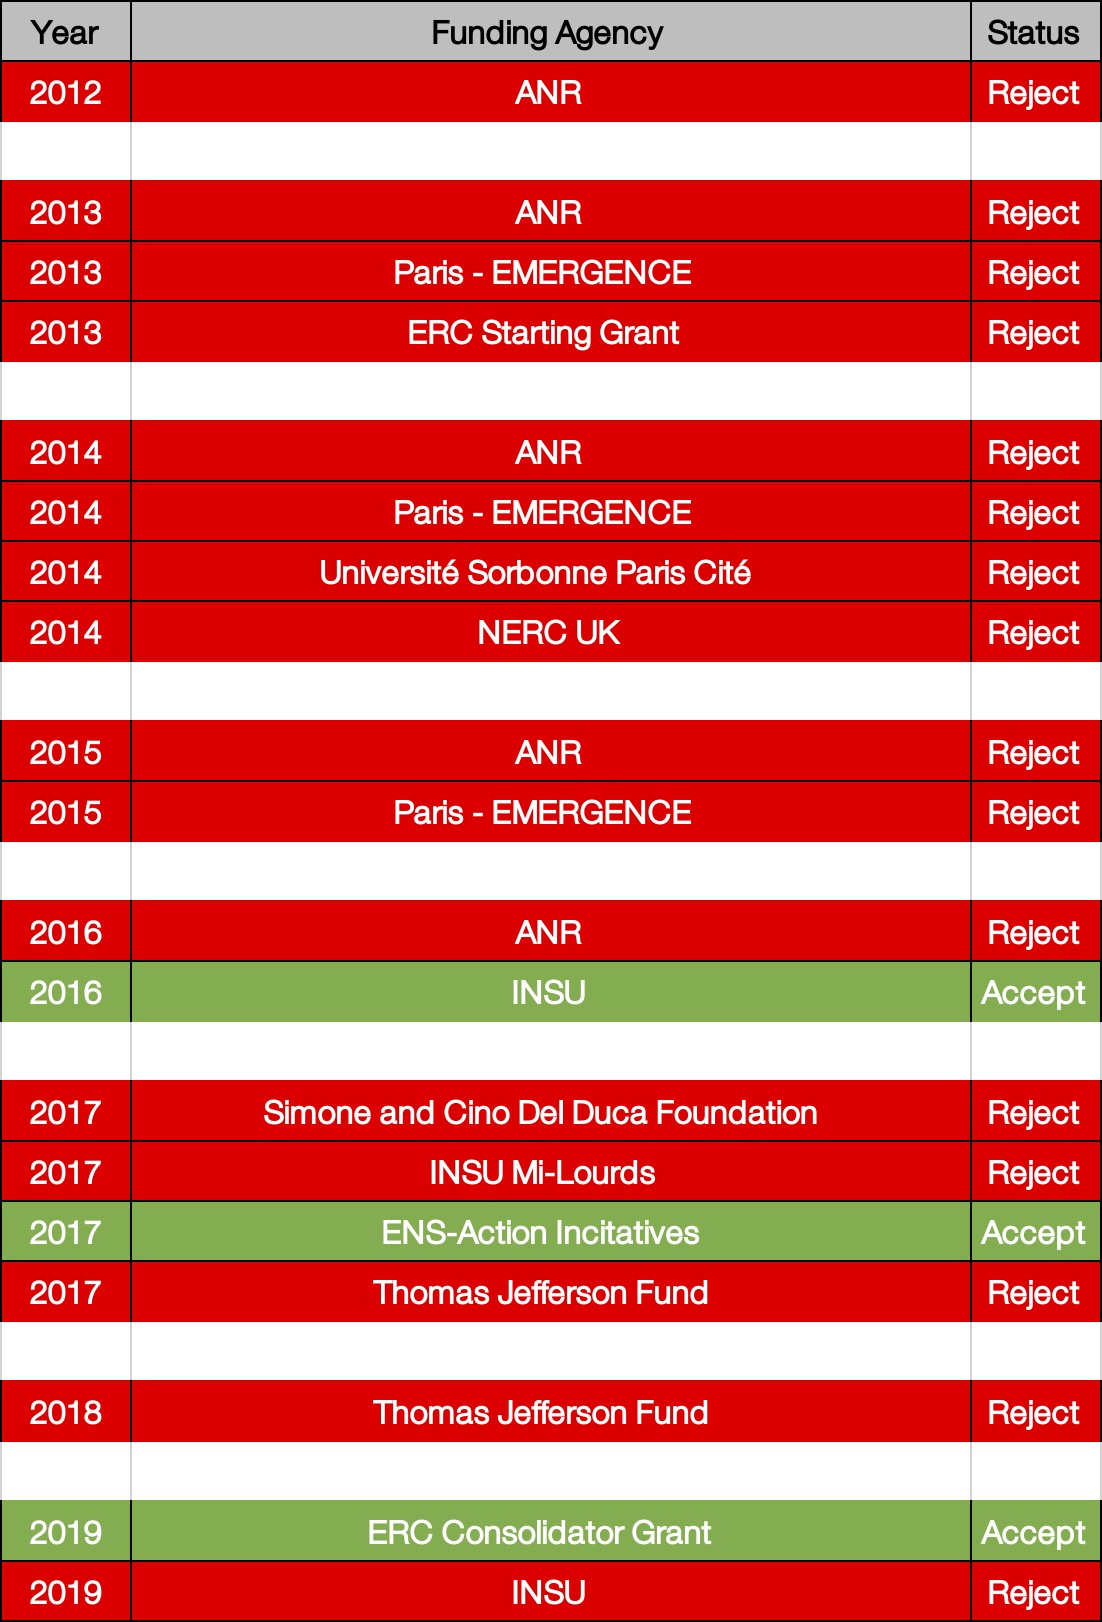
\includegraphics[width=0.5\textwidth]{proposals.jpg}
%  \end{center}
% \vspace{15pt} 
%\end{figure}
%}
%%%%%%%%%%%%%%%%%%%%%%%%%%%%%%%%%%%%%%%%%%%%%%%%%%%%%%%%%%%%%%%%%%%%%%%%%%%%%
\vfill{\scriptsize \hfill \today}
\end{document}